% Este documento contiene el índice del manuscrito de la tesis.
%\documentclass[12pt,a4paper]{report}
%\usepackage{graphicx}
 
%\title{Introduction}
%\author{Claudia Guti\'errez}
%\date{ January 2018}


%\begin{document}

%\maketitle

%\tableofcontents{}

%%%%%%%%%%%%%%%%%%%%%%%%%%%%%%%%%%%%%%%%%%%%%%%%%%%%%%%%%%%%%%%%%%%%%%%%%%%%%%%%%%%%%%
\part{Introduction\label{cha:intro}}

%\section{Transversalidad}

% La ciencia aplicada o aplicación de la ciencia, ha evolucionado las sociedades a través de la conexión de los estudios de ciencia básica con los ingenios que implementaban el conocimiento estructural al día a día de los individuos. La construcción del puente entre los estudios fundamentales y su adaptación/evolución para el desarrollo de las sociedades, ha sido cuestión de una interpretación (y por lo tanto de intérpretes) capaz de econtrar el lenguaje adecuado para intercambiar este conocimiento.

%% Applied science has made societies evolved trough the linked between the basic science and the 'ingenios' that implement the structural knowdlege to the individual daylyligde. The bridge between the fundamental studies and its evolution or transformation into something applied for the societies development, has to be with the interpretation (so interpreters) that have been able to find the accurate languafe to exchange this knowdlege. %%

 % Esta transversalidad entre las disciplinas básicas de la física, la química o la biología con distintas acepciones prácticas, la mayoría de ellas recogidas bajo el paraguas de las ingenierías, desemboca ineludiblemente en una transformación de lo abstracto en lo tangible con la premisa o el ideal de mejorar el bienestar de las sociedades presentes y futuras. 

% Es sin embargo muy probable, que esta concepción de la aplicación científica haya desembocado en el mayor problema al que hacer frente desde.Siendo este antropocentrismo parte del problema, y no de la solución. Jorge Wasenberg escibe en su libro, ``el pensador intruso'' en referencia a la evolución de la ciencia y el progreso subyacente lo siguiente:

% ``Existen sobre todo dos vicios que tienden a inyectar ideología precocinada en la ciencia. Una de ellas se basa en las distintas formas de antropocentrismo y consiste en situar instintivamente al sujeto del conocimiento en el centro del cosmos. La historia del conocimiento es testigo: cada vez que barremos el Yo del centro del escenario el conocimiento avanza, y avanza sólo por ello.''

% Sin caer en lo pretencioso, este trabajo contribuye a la imbricación entre la ciencia del cambio climático y la tecnología renovable de producción eléctrica con mayor potencial a día de hoy, la solar fotovoltaica.

\chapter{Context and introduction}

\epigraphfontsize{\small\itshape}
\epigraph{''Begin at the beginning,'' the King said gravely, ''and go on till you
come to the end: then stop.''}{--- \textup{Lewis Carroll}, Alice in Wonderland}

\section{A changing world} 

% Ideas a desarrollar:

% * Un mundo en constante evolución.
% * Cambio climático
% * Transición energética global
% * Cambios sociales/políticos.
% * Migraciones

Se dice que nada es permanente excepto el cambio. Nos encontramos en un mundo en constante evolución donde inevitablemente algunos de los cambios que nos acontecen nos sobrepasarán sin que seamos capaces de adaptarnos a ellos. Mientras, otros pasarán desapercibidos a nuestros ojos por su lentitud o por no encontrarse en el centro de nuestras preocupaciones. Resulta paradójico pensar que algunos de esos cambios provocados por el ser humano, consciente o incoscientemente, con voluntad o por equivocación, obligarán al mismo como espcecie a resistir y adaptarse frente a las consecuencias de aquello que ellos mismos generaron. 

El desarrollo y la evolución de los pueblos ha estado ligado desde la primera Revolución Industrial a un incremento en la demanda de energía. El uso de los combustibles fósiles desde la invención de la máquina de vapor ha cambiado la forma de vida de las sociedades. Asociado a este crecimiento, las emisiones de gases de efecto invernadero y su concentración en la atmósfera se han disparado con respecto a la época pre-Industrial [ref]. El calentamiento global, con su origen en las actividades humanas, supone uno de los mayores retos de adaptación para el ser humano. El carácter anisotrópico de los impactos asociados al cambio climático pone a prueba la solidaridad con las comunidades más vulnerables y menos responsables en este dilema.[ref]

Para algunos estamos sumergidos en lo que ha sido descrito como una Tercera Revolución Industrial (ref), un proceso de desarrollo científico-tecnológico exponencial, donde convergen el desarrollo de las tecnologías renovables con el uso masivo de las nuevas tecnologías de la comunicación. La transición energética en marcha debería ser la respuesta a una demanda de una ciudadanía comprometida que encuentra en estas tecnologías una alternativa y una respuesta a los problemas medioambientales y sus consecuencias asociadas. 

El contexto actual está caracterizado por una avanzada globalización donde se han eliminado fronteras gracias al desarrollo de las comunicaciones a la vez que se creaban muros físicos para reducir los movimientos reales de personas. El crecimiento de la población y el aumento indefinido de la demanda de recursos para sustentar un sistema basado en el crecimiento continuo provoca conflictos geopolíticos y el agotamiento de estos recursos naturales. Las crisis humanitarias se suceden y los pueblos migran de manera masiva del sur hacia el norte huyendo de las zonas de conflicto.[ref] 

Para poder abordar las necesidades humanas en una coyuntura de crisis global, es necesario un cambio de paradigma. Este cambio debe pasar por reconocer la interdependencia entre la humanidad y los distintos ecosistemas y seres vivos, así como reconocerla importancia intrínseca de la naturaleza en sí misma. En 1962 Thomas Khun en su obra ``La Estructura de las Revoluciones Científicas'' escribió que un cambio de paradigma no ocurre realmente hasta que sus adheridos son reemplazados por una nueva generación. Habrá por lo tanto que esperar para ver el desenlace de este cambio de paradigma, esperando que no sea demasiado tarde.


%* Entrelazamiento de todas estas cuestiones.
%* El conocimiento puro + el conocimiento aplicado: obligación de la ciencia a ser en la medida de lo posible aplicada a solucionar problemas de las distintas sociedades. Justicia social. Más si estos problemas han sido creados por el ser humano.


%Applied science has made societies evolved through the link between the basic science and the implementation of this structural knowdlege to the individual dailylife. The bridge between the fundamental studies and its evolution or transformation into something applied (useful) for the societies development is been a matter of interpretation or 'translation' (so interpreters/translator) to find the accurate language to exchange this knowdlege.

% Esta transversalidad entre las disciplinas básicas de la física, la química o la biología con distintas acepciones prácticas, la mayoría de ellas recogidas bajo el paraguas de las ingenierías, desemboca ineludiblemente en una transformación de lo abstracto en lo tangible con la premisa o el ideal de mejorar el bienestar de las sociedades presentes y futuras.

%Transversality between the fundamental disciplines of physiscs, chemistry or biology and their different applied branches, most of them under the umbrella of engenieering, end unavoidably into a transformation from the abstraction to the tanglible with the premise or ideal of improving wellbeing of present and future societies.

% Es sin embargo muy probable, que esta concepción de la aplicación científica haya desembocado en el mayor problema al que la humanidad tiene que hacer frente desde su existencia, el cambio climático. Siendo este antropocentrismo parte del problema, y no de la solución. Jorge Wasenberg escibe en su libro, ``el pensador intruso'' en referencia a la evolución de la ciencia y el progreso subyacente lo siguiente:

% Nevertheless, it is very likely that this conception of the scientific application had lead to the most challeging problem that humanity has to face from its existance, climate change, being this anthropocentrism part of the problem and not of the solution.

%In his book ``El pensador intruso'', Jorge Wasengber wrote about the evolution of science and the underlying progress what follows: 

%'There are above all two vices that tend to set 'pre-cooked' ideollogy into science. First is base on different kinds of anthropocentrism and consist in put the knowdlege subjet into the cosmos's center. The history of knowdlege is the witness: each time we 'barremos' the 'I' from the spot, the knowdlege progresses and only because of it.'
% ``Existen sobre todo dos vicios que tienden a inyectar ideología precocinada en la ciencia. Una de ellas se basa en las distintas formas de antropocentrismo y consiste en situar instintivamente al sujeto del conocimiento en el centro del cosmos. La historia del conocimiento es testigo: cada vez que barremos el Yo del centro del escenario el conocimiento avanza, y avanza sólo por ello.''

% Sin caer en lo pretencioso, este trabajo contribuye a la imbricación entre la ciencia del cambio climático y la tecnología renovable de producción eléctrica con mayor potencial a día de hoy, la solar fotovoltaica.

\section{Renewable Energy}

\subsection{Concept of energy}
El concepto físico de energía se define como la capacidad que tiene un sistema para realizar un trabajo, clasificando las distintas formas de energía en dos grandes grupos: la energía cinética, relacionada con el movimiento del sistema, o la energía potencial, que atiende a la posición de mismo. En esta clasificación fundamental encontramos que la energía mecánica, electromagnética o térmica son formas de energía que se engloban dentro de la energía cinética, mientras que la energía química (de la cual es un subtipo la energía nuclear) o la energía potencial gravitacional (como es el caso de las centrales hidroeléctricas) se encontrarían dentro de la energía potencial.

%The physics concept of \textit{energy} is defined as the capacity of a system to perform a work and it is divided in two groups: kinetic energy, that is related to the movement of the system, and the potential energy, related to its position. For this fundamental classification, mechanical energy, electromagnetic and thermal energy are encompassed in the kinetic energy group, while the chemical energy or the gravitational potential energy, as it is the case of hydropower,  are inside the potential energy group.

\subsection{Types and classification}
Es elemental para nuestro estudio delimitar la diferencia entre formas y fuentes de energía. Las fuentes de energía son definidas como aquellas a partir de las cuales la energía 'útil', directamente aplicable para su finalidad (sea esta el movimiento, la producción de electricidad o los distintos proc
esos metabólicos en el ser humano), puede ser extraída directamente o mediante algun proceso de transformación.

% It is elementary to this work to delimit the differences between kinds and sources of energy. Sources of energy are defined as those from which useful energy can be extracted, either directly to is end (being this one movement, elecgricity production or matabolic processes) or through some transformation process.

En el contexto del consumo energético de nuestras sociedades, denominaremos fuentes de energía primaria a aquellas a partir de las cuales obtendremos la energía final, tras un proceso de extracción/transformación y transporte. Atendiendo a esto podemos considerar energía primaria a los combustibles fósiles, la energía hidráulica, la energía solar o la biomasa. Estas fuentes de energía primaria proporcionarán la energía final que en muchas ocasiones será en forma de electricidad (salvo aquella destinada al transporte).

%Así, los combustibles fósiles son una fuente de energía, puesto que su energía 'útil' debe ser extraída. Es decir, extraemos la energía química contenida en los combustibles fósiles y necesitamos ciertos procesos de transformación entre la energía potencial de una masa de agua elevada que termina pasando a través de una turbina para obtener electricidad. Algunos ejemplos de fuentes de energía son los combustibles fósiles, la energía solar o la biomasa.

% It is basic in this work to delimit the difference between \textbf{energy kinds} and \textbf{energy sources}. The last are defined as those from where the \textit{useful} energy, directly applicable to its ends (electricity production, mechanical movement, metabolic processes...), can be extracted directly or by some transformation process. Thus, fossil fuels are a source of energy and some transformation are needed to extract the useful energy. 

Aparece de manera natural la clasificación de estas fuentes de energía primaria según su origen renovable, siendo estas últimas aquellas fuentes inagotables. El sol, a pesar de su indiscutible finitud,  es considerado una fuente inagotable de energía debido a la diferencia entre la escala temporal de la vida humana y la vida de la estrella a la que nos refereimos, muchos órdenes de magnitud mayor.

\subsection{History and evolution}

El uso de la energía renovable ha acompañado el desarrollo de la humanidad desde tiempos remotos. Desde la utilización de la biomasa para generar energía térmica para calentarse, hasta la transformación de la energía eólica en energía mecánica en los molinos tradicionales o en la navegación. Solo hacia la mitad del siglo 19, con la invención de la máquina de vapor, comenzó la utilización de los combustibles fósiles de manera masiva y con ello lo que se denominó la Revolución Industrial. Este periodo supuso un gran desarrollo en términos tecnológicos así como en la evolución del bienestar de las sociedades, al menos de aquellas que hemos llamado, occidentales.

Sin embargo, este desarrollo trajo asociado un aumento de la demanda de combustibles fósiles que ha crecido de manera explonencial, durante el siglo 20y ha generado numerosos conflictos. Las sociedades cada vez más demandantes de energía han crecido a espaldas de la realidad de sustentar su desarrollo en recursos finitos y distribuidos de manera desigual en la Tierra.

El primer impulso para diversificar las fuentes de energía primaria no tuvo lugar hasta los años 70, con la primera crisis del petróleo [ref]. El embargo de los países productores de petróleo tuvo grandes consecuencias económicas en los países importadores, lo que provocó que algunos comenzaran a considerar nuevas formas de energía para asegurar su estabilidad y abastecimiento.

En las últimas décadas, además de factores socioeconómicos y geopolíticos que han llevado a la necesidad de limitar la dependencia del petróleo en los países importadores, el impulso para el crecimiento exponencial de estas tecnologías alternativas, ha venido provocado por el gran descenso en sus costes, que tiene su origen sobre todo en el fomento de políticas ``verdes'' impulsadas por distintos organismos y gobiernos [IPCC] y que han generado un círculo virtuoso alrededor de estas tecnologías. El descenso en los costes gracias a las políticas de support y con visión a largo plazo, ha favorecido, a su vez, una mayor implantación de objetivos nacionales en la instalación de plantas de generación renovable para combatir el cambio climático. En 2017 más de 170 países habían establecido objetivos de generación renovable (IRENA 2017).

En 2018 las energías renovables ya suponen un $55\%$ de la energía final consumida según un informe de REN21, con un porcentaje del $27\%$ en generación de calor y un $25\%$ de electricidad. El transporte, en cambio, sigue siendo el sector con menor porcentaje de renovables con sólo un $3\%$. 

\begin{itemize}
\item Algunas estadísticas más sobre renovables  
\item Remarcar el crecimiento de la fotovoltaica
\item Terminar con: los escenarios futuros estarán determinados principalmente por 3 factores: un aumento en la demanda dada sobre todo por los países en desarrollo, una mayor electrificación y un descenso en el consumo de los combustibles fósiles.  
\end{itemize}


\section{Photovoltaic Energy}

La energía fotovoltaica tiene como fundamento la conversión de energía solar inidente del sol en energía eléctrica. Este proceso se realiza mediante sistemas denominado fotovoltaicos cuya unidad básica encargada de transformar la radiación solar en electricidad es la \textbf{célula solar}.

\subsection{Union P-N}

El fundamento físico de la célula solar se basa en lo que se conoce como \textbf{unión P-N}: un dispositivo que pone en contacto dos semiconductores extrínecos, también llamados dopados, de tipo P y de tipo N.

Los semiconductores de tipo N son semiconductores a los que se les añaden impurezas: átomos con un número mayor de electrones de valencia que el semiconductor original. De esta manera, existe un exceso de electrones, o \textbf{portadores} de carga negativa, en un cristal tipo N. Al integrar el nuevo átomo en la red, Los electrones extras pasan a la banda de conducción del semiconductor, permaneciendo en la red la carga positiva asociada. A esta carga positiva se le denomina \textbf{hueco} o vacante. En un semiconductor tipo N la concentración de electrones será mayor que la concentración de huevos, siendo el portador mayoritario.

En un semiconductor de tipo P, el proceso de dopaje consiste en añadir a la red cristalina algunos átomos con un número menor de electrones que el semiconductor original. Ahora, la densidad de huecos en la red es mayor que la de electrones. 

% En un semiconductor no dopado cuando los electrones de la banda de valencia adquieren la energía suficiente para pasar a la banda de conducción, estos dejan una vacante o hueco libre. Mediante la acción de un campo externo, los electrones que se encuentran en la banda de conducción pueden desplazarse junto con los electrones que han quedado en la banda de valencia, que pueden moverse debido a los huecos generados por los electrones más energéticos. El movimiento de los electrones en la capa de valencia origina a su vez un desplazamiento de las vacantes, lo que puede verse como un desplazamiento de carga positiva en sentido opuesto. A los electrones de la banda de conducción y huecos de la banda de valencia los denominamos portadores. Cuando un semiconductor intrínseco se encuentra en equilibrio térmico la concentración de portadores 'p' y 'n' es igual.

La unión P-N pone en contacto los dos semiconductores provocando un desequilibrio debido a la diferencia en la concentración de portadores de los dos semiconductores. Esta diferencia en la densidad de portadores origina un proceso de difusión de un lado a otro de la unión, consistente en un movimiento de huecos hacia el lado 'n' por la banda de valencia y de portadores tipo 'p' hacia el el lado opuesto por la banda de conducción. Si los portadores no estuvieran cargados eléctricamente, este proceso de difusión continuaría hasta el equilibrio. Debido a su carga eléctrica, el movimiento de difusión de los portadores hace que al recombinarse en el lado opuesto,  los iones anclados en la red originen un campo eléctrico desde el semiconductor tipo N al P. Este campo tiene  genera lo que se conoce como corriente de arrastre, que se opone a la corriente de dufusión de portadores. Ahora, el equilibrio se alcanzará cuando los procesos de arrastre y difusión se igualen.

Cuando se ha alcanzado el equilibrio, en la zona más cercana a la unión, que se conoce como \textbf{zona de carga del espacio}, los portadores minoritarios se han recombinado y en ella sólo están los iones cargados ligados a la red. El campo eléctrico originado por los iones crea una diferencia de potencial denominado, potencial termodinámico, que impide a los portadores mayoritarios pasar de un cristal a otro.

\subsection{Polarized P-N}

Para poder hacer circular corriente a través de la unión P-N es necesario romper el equilibrio y para ello será necesario reducir el potencial termodinámico. La manera de hacerlo consiste en aplicar una diferencia de potencial entre los extremos del cristal. Si el lado P tiene una tensión positiva con respecto al lado N, la unión está polarizada en directa y en inversa en el caso contrario. Con la polarización directa, disminuye la barrera de potencialn y con ello la corriente de arrastre que ya no puede compensar la difusión. Ahora, los portadores de cada lado pueden atravesar la zona de carga del espacio y llegar al otro lado, donde son los portadores minoritarios. Ahora, el proceso de difusión provoca dos corrientes con sentidos opuestos pero de cargas diferentes, por lo que no se anulan y crean una corriente aprovechable.

Cuando la unión P-N está polarizada en inversa, es decir que el lado P tiene una tensión negativa, el potencial termodinámico aumenta y no circulará ninguna corriente aprovechable.

Los procesos de generación de corriente en la unión P-N pueden resumirse en la ecuación de Shockley \ref{eq:shockley} que define la corriente generada por un diodo. El diodo es el dispositivo electrónico que se basa en el funcionamiento teórico de la unión P-N. En \ref{eq:shockley} $I_0$ es la corriente de saturación del diodo en oscuridad, $V$ la tensión aplicada y $m$ un factor para ajustar al funcionamiento real y $V_T$ el potencial térmico.

\begin{equation}
  I_{D}=I_0\cdot [e^{{V}\over {m\cdot {V_{T}}}}-1]
\label{eq:shockley}
\end{equation}

\subsection{Solar Cell}

Cuando la unión P-N es iluminada, la energía de la luz incidente puede ser absorbida por los electrones del semiconductor que pasan entonces  a la banda de conducción, por el fotoeléctrico. En este proceso, se producen portadores de carga, pares electrón-hueco que son conducidos por el campo eléctrico de la unión generando una corriente. Esta corriente puede denominarse ``fotocorriente'',$I_L$, y será de sentido opuesto a la corriente del diodo.

La ecuación \ref{eq:Isolar} determina la corriente genearada por una célula solar iluminada:

\begin{equation}
  I=I_L - I_0\cdot [e^{{V}\over {m\cdot {V_{T}}}}-1]
\label{eq:Isolar}
\end{equation}

La fotocorriente generada dependerá en primer lugar de la energía de la luz incidente. Si su frecuencia tiene es demasiado baja, la luz no tendrá la energía suficiente para romper enlaces y atravesará el material sin ser absorbido. Por ello, no toda la luz incidente será aprovechable para generar corriente, sino que existirán pérdidas por transmisión, así como otras pérdidas por reflexión o recombinación de algunos de los portadores.

\subsection{Photovoltaic system}
Un sistema fotovoltaico transforma radiación en energía eléctrica.

\section{Links between climate and renewable energy}

El sector energético en general y las tecnologías renovables en particular son altamente dependientes del estado de la atmósfera. La cantidad de recurso disponible en cada momento determinará, no sólo la energía final que podemos generar con las distintas tecnologías (eólica, fotovoltaica etc.), sino en muchos casos, afectará a la demanda eléctrica en situaciones meorológicas de (por ejemplo) olas de frío o extremo calor. Por ello el mercado energético y los diferentes agentes del sector, así como la necesidad de que la generación y la demanda eléctrica estén balanceadas en todo momento, necesitan de información meteorológica de alta calidad y resolución. Con ello será posible establecer y predecir la cantidad de energía que se puede generar con cada tecnología renovable. 

Por otro lado, las condiciones meteorológicas afectan de manera indirecta en otros muchos aspectos. Por ejemplo, el mantenimiento de un parque éolico offshore es un proceso extremadamente complejo debido a la accesibilidad de los aerogeneradores. Conocer de antemano la predicción meteorológica es necesario para planificar y evitar poner en riesgo a las personas implicadas.  

Aunque las fases de operación o mantenimiento en las plantas de generación eléctrica constituyen uno de los núcleos más importantes del proyecto, es necesario considerar también algunas etapas que requieren de escalas temporales más largas. En primer lugar, para poder establecer la idoneidad de una planta de generación renovable, se establece una fase de evaluación del recurso o evaluación del potencial. En este periodo, se analizarán series temporales largas que sean representativas del recurso disponible en una zona. Esta etapa permite a los promotores establecer la energía máxima disponible que serán capaces de vender en el mercado eléctrico y será necesaria para poder establecer una financiación adecuada.

En el contexto actual de calentamiento global, la relación entre energía y clima ha estado ligada habitualmente al impacto que una mayor participación de las renovables en el mix de generación puede provocar en él, considerando la posible reducción de las emisiones de gases de efecto invernadero de origen antopogénico por esta vía. Sin embargo, el hecho de que el cambio en el clima puede a su vez provocar un cambio en la disponibilidad o distribución de los recursos renovables, así como en los patrones de demanda eléctrica, debe ser investigado en profundidad. [JRC report:Climate modelling and renewable energy resource assessment].

\begin{figure}[h!]
\centering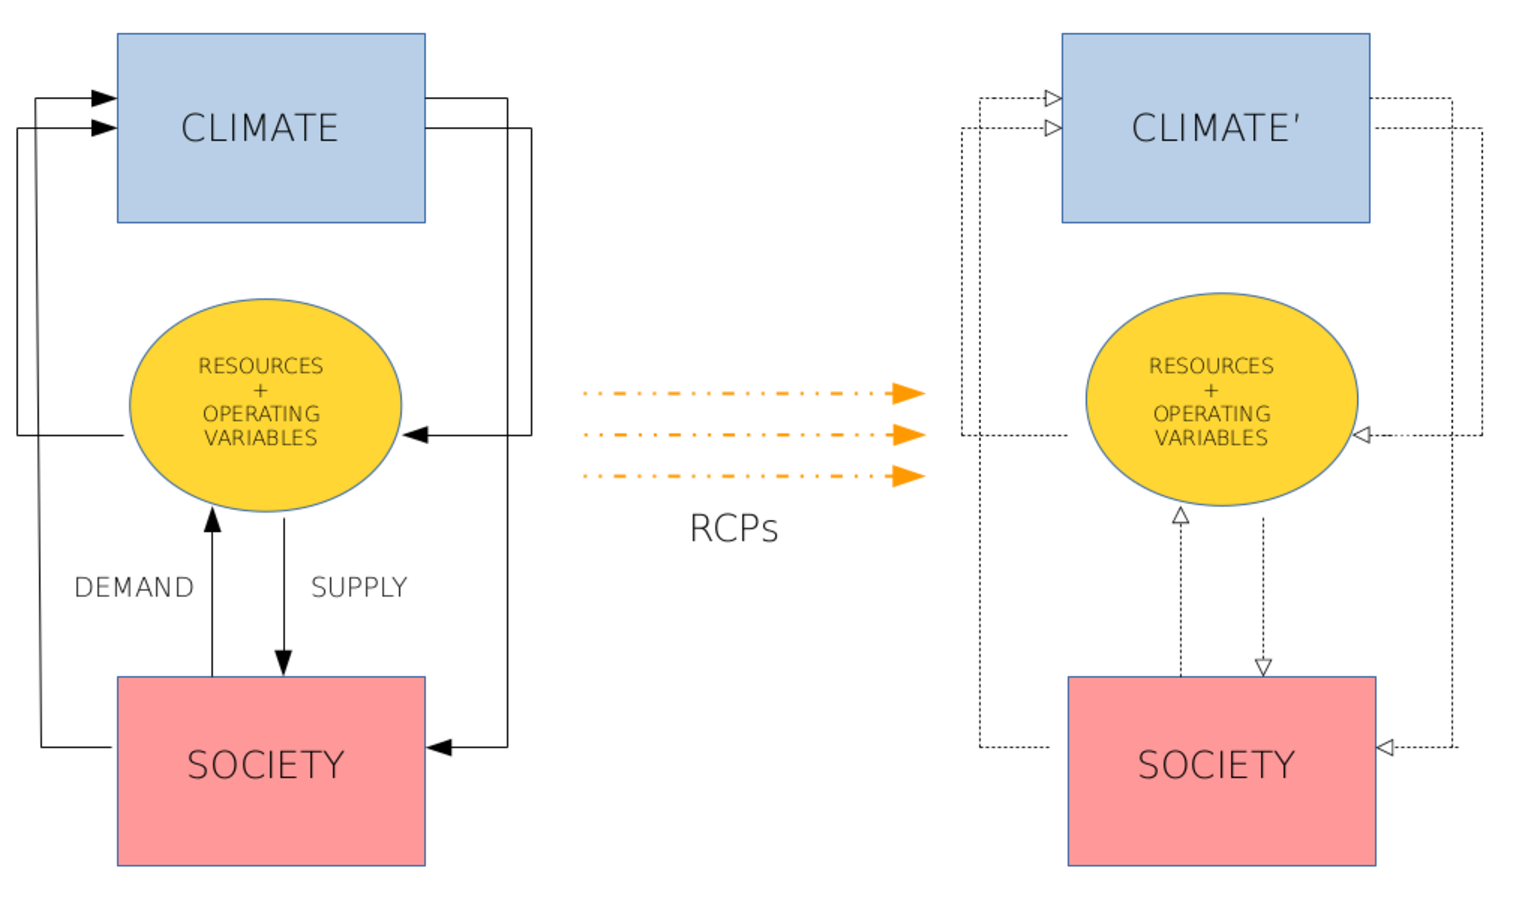
\includegraphics[width=0.6\textwidth]{figs/esquema.pdf}
\caption{Scheme: }
\label{fig:feedback}
\end{figure}

Debido a las características intrínsecas de los recursos renovables relacionadas con su alta variablidad espacio-temporal, el sector energético demanda análisis y conocimiento profundo acerca de éstas caracteríticas en distintas escalas temporales. Esto, ayudaría a una mayor integración de las mismas así como a la mejora en la planifición, poniendo cada vez más relevancia en las escalas climáticas.

En la figura... están representados diversos eventos meteorológicos y climatológicos que afectan a la generación energética. El eje 'x' representa las distintas escalas temporales en las que ocurren estos eventos. Es interesante destacar, aunque no es el tema principal de esta investigación, la relevancia de la escala estacional y sub-estacional para la operación de las plantas energéticas de tipo renovable. La mejora en la predicción climática en estas escalas repercutirá de forma directa en la planificación de la operación y mantenimiento, así como ayuda en la gestión por parte del operador de red y mercado. Por ejemplo, conocer con antelación si un otoño va a ser especialmente lluvioso, sirve para predecir la cantidad de electricidad que se puede producir con las centrales hidroeléctricas, haciendo el sistema mucho más eficiente y fiable. 

Uno de los problemas asociados al posible cambio en el medio-largo plazo de los recursos renovables, como puede ser el eólico, es la posible pérdida de rentabilidad de algunos proyectos que actualmente se encuentran en fase final de su vida. La repotenciación de estos proyectos con tecnologías más actualizadas, como puede ser la sustitución por turbinas eólicas de mayor potencia, junto con la prolongación de las concesiones de explotación del proyecto [ref] son una de las opciones que se dan en aquellas plantas de generación que se instalaron hace casi dos décadas. Los cambios en el recurso pueden cambiar las condiciones del proyecto no sólo por la modernización de la maquinaria y tecnología empleada, sino por el recurso disponible en la misma zona.

La bancabilidad[ref] de un proyecto renovable depende de dos factores: en primer lugar su recurso y en segundo lugar, sus beneficios. Los beneficios obtenidos por el proyecto renovable dependerán del periodo de operación y de la cantidad de energía suministrada en este tiempo. Por ello, una evaluación adecuada, no sólo del recurso disponible a lo largo de todo el proyecto, sino de su variabilidad y de las posibles tendencias, es necesario a lo largo del ciclo de vida de la planta, que puede alargarse hasta 30 años[ref].

% !! escalas climáticas: ¿es importante la repotenciacion? tener en cuenta esto? mismo recurso en el futuro?
% !! infraestructuras y extremos climáticos.
\subsection{Climate services}

Con la creciente demanda de información por parte del sector energético de predicciones y proyecciones climáticas, aparece de manera natural la creación de los servicios climáticos para sistematizar, de alguna manera la información necesaria para los distintos stakeholders. 

Como puede observarse en la figure \ref{fig:feedback}, los procesos de interacción entre la sociedad y las variables involucradas en la generación de energía son de doble sentido. Por un lado el abastecimiento dependerá de la disponibilidad de los recursos y por otro, la demanda está directamente influenciada por estos factores climáticos. Teniendo en cuenta esto, el desarrollo de los servicios climáticos debe basar la mejora de sus modelos y por lo tanto, de los productos ofrecidos en estas dos premisas.

La información climática en el sector energético es especialmente relevante para las descisiones estratégicas y la evaluación de riego, las operaciones de trading o la planficación de la operación y el mantenimiento en las plantas de generación (especialmente) renovables.

Es relevante, aunque no es el tema de esta tesis, decir que también otros tipos de generación no renovable pueden beneficiarse de esta información y estar afectados de manera importante por algunos eventos climáticos. Por ejemplo, el aumento de temperatura del aire puede provocar una subida en la temperatura de los ríos, que ocasionalmente repercute en la operación de las plantas nucleares. En estos casos, estas plantas se ven afectadas porque no pueden continuar on las operaciones de refrigeración de los reactores (ref). 

%\section{Resource assessment}
\section{Climate change and the Mediterranean area}

% \begin{itemize}
% \item Cambio climático de origen antropogénico a escala global. Aumento de la temperatura global.
% \item Los impactos del cambio climático ocurren en escalas locales o afectan de manera local a distintas comunidades y poblaciones de una forma desigual, relacionada también con su capacidad de adaptación y resiliencia.
% \item Por las razones mencionadas arriba, la respuesta a los diferentes impactos de cambio climático deben adoptarse de manera local, a pesar de que el consenso sobre la urgencia de actuación sea global y se adopten compromisos globales comunes.
% \item La mitigación de los grandes impactos ocurre en escala regional/local.
% \end{itemize}

El sistema climático ha variado continuamente y de manera significativa a lo largo de la historia de la Tierra. Las variaciones del clima puede explicarse debido a factores o forzamientos externos y la respuesta del sistema climático a los mismos o, por otro lado, puede ser la causa de inestabilidades internas y relaciones no lineales entre los distintos componentes del sistema.

Los distintos forzamientos de origen externo pueden ser factores astronómicos, como los cambios en la intensidad de la radiación solar o en los parámetros orbitales o por otro lado, factores terrestres como la composición de la atmósfera debido a la actividad humana, por ejemplo, o cambios en la superficie terrestre debido al uso de la misma. 

Algunas variaciones del sistema climático ocurren de manera independiente de los forzamientos externos. Estas variaciones tienen su origen en las distintas interacciones no lineales entre los componentes del sistema climático y dan como resultado la variabilidad natural del sistema climático. 

Desde la revolución industrial la Tierra ha experimentado un aumento de la temperatura global que no es posible explicar mediante los forzamientos externos 'naturales'  del clima como cambios en la actividad solar o en las emisiones volcánicas (Bindoff et al, 2013), ni forma parte de la variabilidad natural del sistema. El IPCC en su último informe, asegura que la actividad humana y en concreto las emisiones de efecto invernadero generadas desde la Revolución Industrial (1850) son responsables del cambio climático que ha generado el ascenso de temperatura global y que ha hecho que probablemente los 30 años entre 1983-2012 hayan sido los más cálidos en los últimos 1400 años en el hemisferio norte (IPCC). A pesar de la marcada variabilidad interanual (Stocker et al. 2013), el aumento de temperatura con caracter global en las últimas décadas es evidente. [ref de observaciones globales]

Las consecuencias del aumento de temperatura desde un punto de vista físico dependen de la sensibilidad del sistema a los cambios en la concentración de gases de efecto invernadero. Son numerosos los estudios [ref] que se han realizado para intentar cuantificar el impacto que este aumento de temperatura puede tener en los distintos subsistemas a través de los diferentes mecanísmos de retroalimentación que pueden generarse.

A pesar de la característica global del cambio climático, sus consecuencias e impactos son percividos a escala local y regional. Estos impactos afectan a comunidades y poblaciones de manera desigual dependiendo de su capacidad de adaptación y resilencia. Por ello, la respuesta desde un punto de vista socio-económico para mitigar estos efectos, tiene que venir dada en esta escala, aunque exista consenso sobre la urgencia de actuación y se adopten compromisos comunes.

Uno de los primeros trabajos que intentaba cuantificar el impacto del cambio climático a escala local fue el de Giorgi et. al 2006. En este trabajo, se utilizaba por primera vez un índice (RCCI) para medir de forma cuantitativa y compara geográficamente las zonas más afectadas por el CC. En este aspecto, el trabajo estaba enfocado desde un punto de vista climático, es decir, el índice mide la sensibilidad del clima en esa zona. En este sentido, el Mediterráneo aparecía como una de las zonas más afectadas y desde entonces ha sido denominado como un hot-spot de CC.

Los ensembles de modelos climáticos proyectan escenarios en los que las principales consecuencias del calentamiento global en el área Mediterránea son un descenso generalizado de las precipitaciones, debido a un aumento de la circulación anticiclónica asociada a un desplazamiento hacia el norte de ``Atlantic storm track''. Las temperaturas proyectadas son inusualmente altas con un ascenso especialmente alto en los meses de verano.


\section{Objectives and sceintific questions}%General scientific question: spatiotemporal behaviour of solar resource and photovoltaic production}

Tras esta introducción se puede definir el principal objetivo de esta tesis que en esencia relaciona cuestiones climáticas con la producción de electricidad con energía solar fotovoltaica. En un contexto de cambio y transición energética, el uso de la tecnología fotovoltaia no ha parado de crecer y los distintos escenarios indican que continuará creciento en un futuro. La varibilidad de los recursos energéticos renovables es una de las principales dificultades en su integración masiva en los sistemas actuales de generación eléctrica, y el impacto de esta varibilidad en escalas climáticas no ha sido estudiado en detalle.

El objetivo será determinar las características espacio-temporales del recurso solar en el área Mediterránea y del potencial o productividad fotovoltaico en escalas climáticas además de determinar el papel de los aerosoles en estas características. Se distinguen 3 capítulos que tratan desde distintas perspectivas este tema.

En el primer capítulo de resultados se analizará una estrategia para regionalizar una unidad geográfica con coherencia desde el punto de vista eléctrico en fucnión de sus características climáticas. En concreto se estudia la Península Ibérica por ser un sistema ``casi aislado'' de manera natural por las dificultades de interconexión con el resto del continente Europeo. 

Por otro lado, en el capítulo 6 se estudia el papel de los aerosoles en la variabilidad del recurso y con ello en la producción. La importancia de los aerosoles en escalas climáticas y su impacto geográfico en este capítulo.

Por último, la importancia de la proyección de los recursos renovables en las condiciones de cambio climático queda reflejada en el capítulo 7 dónde se estudia la posible evolución del recurso solar y el potencial fotovoltaico con respecto a las distintas configuraciones de aerosoles climáticos en los diferentes modelos regionales analizados.

\section{Organization of the manuscript}%\section{General scientific question: spatiotemporal variability of solar resource and photovoltaic production}

The manuscritp is organizded as follows:

The first part contains two chapters: the first one is the Introduction, that aims to overlook the context in which the thesis has been elaborated. In the second chapter it is analysed the main contributions related to the this topic over the literature. It will include the main results about intermittency of PV and how the short-term problems has been managed to go through the long-term problems. After that, the climate change perspective over the area and the main results related to solar resources are presented.

The second part includes two chapters including the Data description and the Methodology used along the studies. In this case it is important to remark that each result's chapter contains the Data and Methodology used for that specific chapter. The contents of this part are related to general description of climate data and models.

Results are presented in the third part.

Finally the fourth part contains a chapter with the main conclusions of the thesis and another chapter that summarizes the main questions emerged from the wotk, which will lead future research.

% \section{State of the art}
% \subsection{From short to long term varibility issues}
% \subsection{Solar radiation data measurements}
% \subsection{Satellite data}
% \subsection{Modelization of solar radiation}
% \section{Identification of knowdlege gaps and approach to the problem}
%\subsection{Spatiotemporal long-term variability in an almost isolated area}
%\subsection{Role of aerosols in the spatiotemporal varibility of the photovoltaic energy production}
%\subsection{Future availability of photovoltaic potential}


\chapter{State of knowdlege\label{cha:state}}
\section{Intermittency of PV}
\section{Variability sources in PV}
\section{From short to long term issues}
\section{Climate Change perspectives for solar resource and photovoltaic potential}

%\end{document}